\section*{Biography Section}
%If you have an EPS/PDF photo (graphicx package needed), extra braces are
%needed around the contents of the optional argument to biography to prevent
%the LaTeX parser from getting confused when it sees the complicated
%$\backslash${\tt{includegraphics}} command within an optional argument. (You can create
%your own custom macro containing the $\backslash${\tt{includegraphics}} command to make things
%simpler here.)

%\vspace{11pt}
%
%{\bf If you include a photo:}\vspace{-33pt}
%\begin{IEEEbiography}[{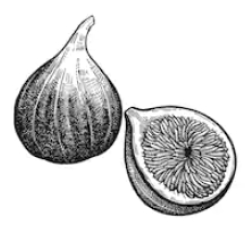
\includegraphics[width=1in,height=1.25in,clip,keepaspectratio]{figures/fig1}}]{Michael Shell}
%	Use $\backslash${\tt{begin\{IEEEbiography\}}} and then for the 1st argument use $\backslash${\tt{includegraphics}} to declare and link the author photo.
%	Use the author name as the 3rd argument followed by the biography text.
%\end{IEEEbiography}
%
%\vspace{11pt}
%
%{\bf If you will not include a photo:}\vspace{-33pt}
%\begin{IEEEbiographynophoto}{John Doe}
%	Use $\backslash${\tt{begin\{IEEEbiographynophoto\}}} and the author name as the argument followed by the biography text.
%\end{IEEEbiographynophoto}

\begin{minipage}{\linewidth}
	\begin{IEEEbiography}[{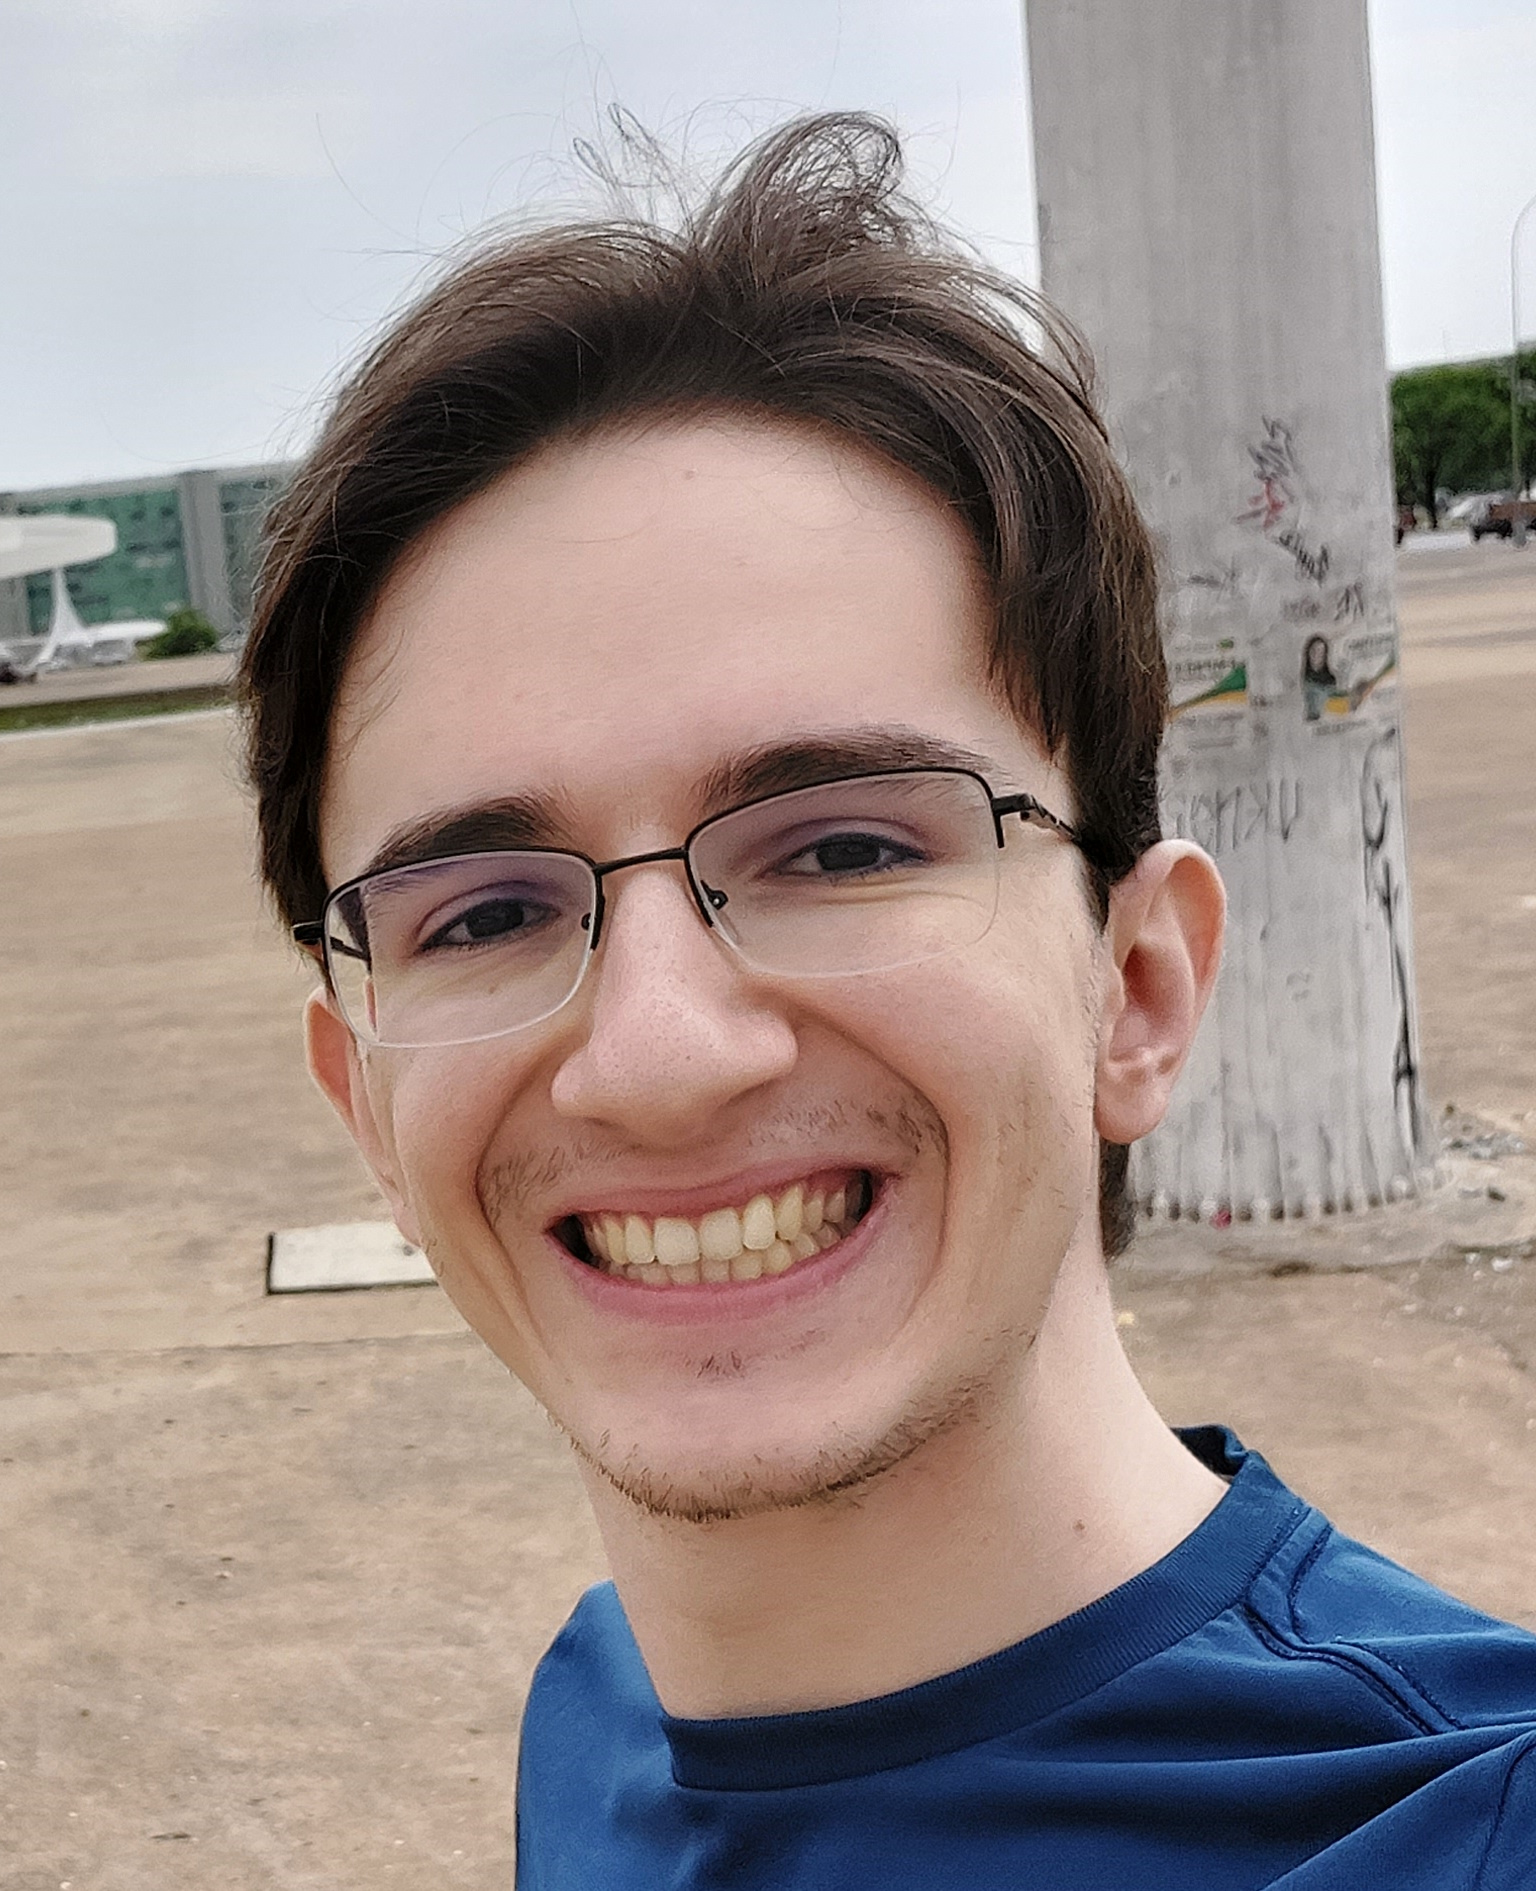
\includegraphics[width=1in,height=1.25in,clip,keepaspectratio]{figures/pictures/vitor}}]{Vitor Probst Curtarelli}
		received the B.Sc. and M.Sc. degrees in Electrical Engineering from the Federal University of Santa Catarina (UFSC), Florianópolis, Brazil, in 2021 and 2023, respectively. From 2023 to 2024 he worked under the guidance of prof. Israel Cohen as an assistant researcher at the Technion - Israel Institute of Technology, in Haifa, Israel. His current research interests are in digital signal and audio enhancement and sensor array signal processing.
	\end{IEEEbiography}
	
	\vspace{11pt}
	
	\begin{IEEEbiography}[{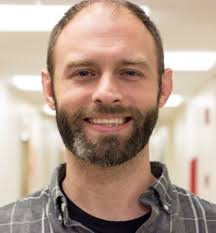
\includegraphics[width=1in,height=1.25in,clip,keepaspectratio]{figures/pictures/israel}}]{John Doe}
		\lipsum[2]
	\end{IEEEbiography}
\end{minipage}